\section{Parallelisation}

Parallel computing has, during the last decade, become a major topic
not only in high-performance computing but in other fields of
computing as well. As it gets tougher and tougher to squeeze in more
circuits in a CPU, the idea of having several CPUs (or CPU cores) is
today not only utilised in super computers but in most modern user
workstations as well.

There are mainly two different hardware setups that has to be
distinguished between in parallel computing. Either the memory is
shared between all or distributed locally at each processing unit
(PU). The former is often referred to as a shared memory and the
latter to a distributed memory computer. An example of a shared memory
computer would be a workstation having two CPU cores sharing the same
RAM. A system using distributed memory could for instance be a super
computing cluster where several computers (nodes) are connected in a
network.

Obvious differences arise in how the processing units may access data
and communicate data between each other.  In the case with shared
memory computers, common address spaces may be used for communication
and for distributed, messages are passed over the network. As a
programmer there is a major difference in how this is done. Since this
is a common task, there exist software for simplifying the
parallelistation of a code. In distributed parallel computing an
interface is defined for how the communication over the network may be
done, this interface is called MPI (Message Passing Interface). There
are several implementations of MPI, one example is Open MPI
\cite{openmpi}. For shared memory computers OpenMP \cite{openmp} is an
API that allows for a rather effortless way of parallelising a code.

An algorithm may in a varying degree be suited for parallelising. If
there is a lot of data dependence or dependencies in general. It may
be difficult to divide the computation in independent tasks on
different PUs. In the case with the algorithm in lattice-Boltzmann,
the algorithm is very well suited for parallelisation. This is often
considered a great strength of the lattice-Boltzmann method. The
main part of the computation is done in the collision step, and a
collision on a node is computed independently of data from other
nodes. In parallelisation of the streaming step however, communication
between nodes are needed. The win in performing the streaming step in
parallel is much smaller than for the collision step. By this reason
and the fact that a shared memory parallelisation using OpenMP is
chosen, only the collision step is parallelised in this work.

The parallelisation was tested for a sample system of $100 \times 100$
nodes with periodic boundary conditions and large number of time
steps. The speedup was measured for different number of parallel
processes used. The result using 2, 5 and 10 respectively cores is
shown in fig. \ref{fig:hpc:para}. The computer used had more than 10
CPU cores. 

\begin{figure}
\begin{center}
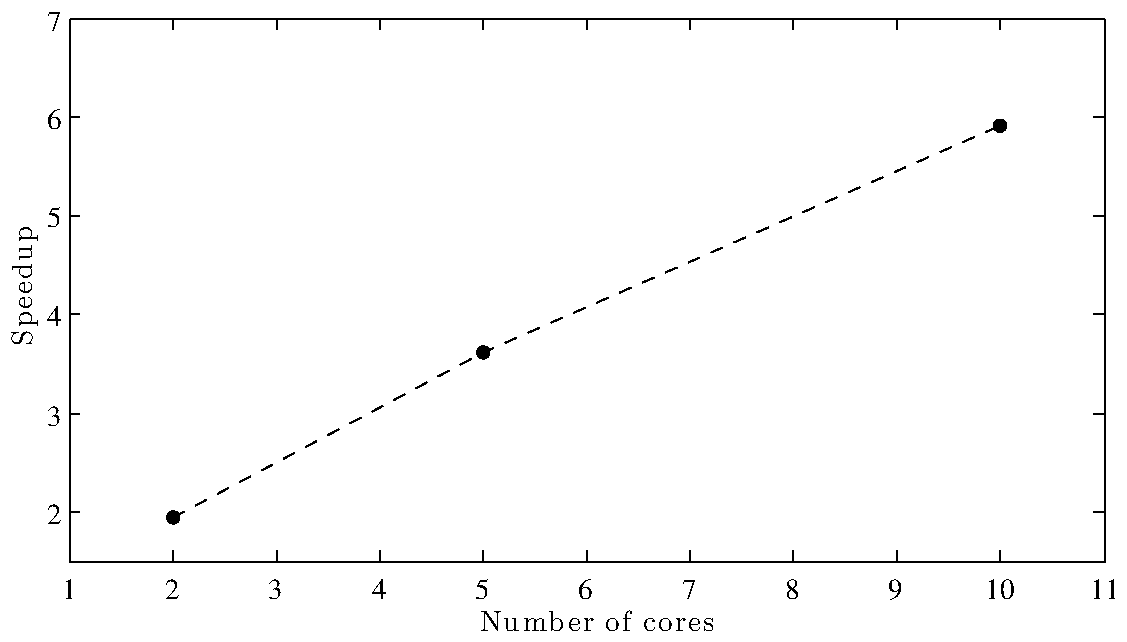
\includegraphics[width=0.9\textwidth]{fig/para.pdf}
\end{center}
\caption[Speedup of the parallelised lattice-Boltzmann code.]{Speedup
    of the parallelised lattice-Boltzmann code. Only the collision
    step with a BGK collision operator and not the streaming step is
    parallelised. The computation was done on a computer with two 12
    cores \texttt{Intel(R) Xeon(R) X5650} CPUs.}
\label{fig:hpc:para}
\end{figure}


\nomenclature{API}{Application Programming Interface}
\nomenclature{MPI}{Message Passing Interface}
